\documentclass[letterpaper]{article}
\usepackage{tikz}
\begin{document}
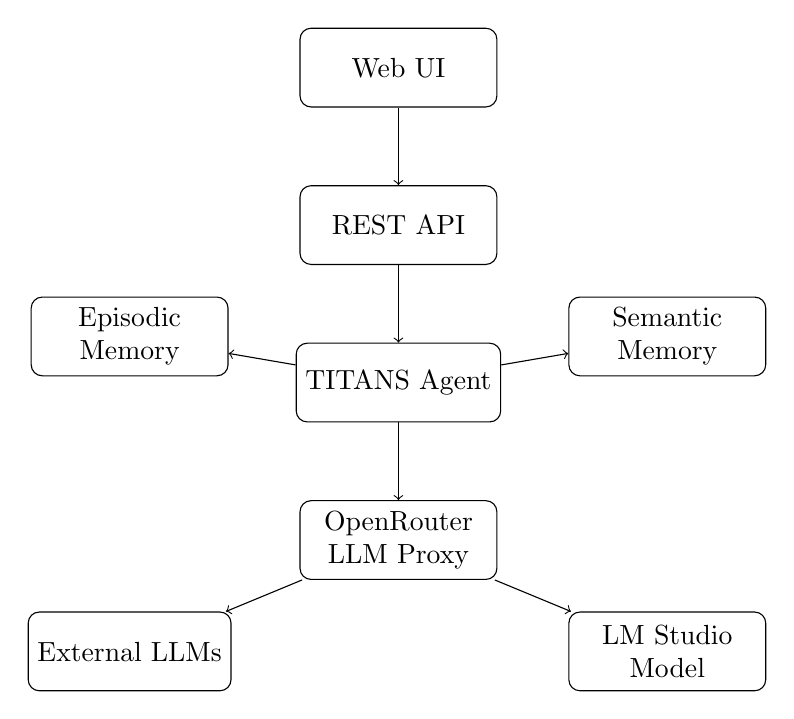
\begin{tikzpicture}[node distance=2cm, box/.style={draw,rectangle, rounded corners, minimum width=2.5cm, minimum height=1cm, align=center}]
  % Nodes
  \node[box] (webui) {Web UI};
  \node[box, below of=webui] (api) {REST API};
  \node[box, below left of=api, xshift=-2cm] (epis) {Episodic\\Memory};
  \node[box, below right of=api, xshift=2cm] (sem) {Semantic\\Memory};
  \node[box, below of=api] (agent) {TITANS Agent};
  \node[box, below of=agent] (openrouter) {OpenRouter\\LLM Proxy};
  \node[box, below left of=openrouter, xshift=-2cm] (gpt) {External LLMs};
  \node[box, below right of=openrouter, xshift=2cm] (lmstudio) {LM Studio\\Model};
  % Connections
  \draw[->] (webui) -- (api);
  \draw[->] (api) -- (agent);
  \draw[->] (agent) -- (epis);
  \draw[->] (agent) -- (sem);
  \draw[->] (agent) -- (openrouter);
  \draw[->] (openrouter) -- (gpt);
  \draw[->] (openrouter) -- (lmstudio);
\end{tikzpicture}
\end{document}